\chapter{Regulamento de Projeto Final}
\label{cha:regulamento}

O processo de submissão e avaliação de projetos finais no curso
de Ciências da Computa\-ção da UECE segue um regulamento que normatiza 
o tipo do conteúdo da monografia, o procedimento para o desenvolvimento 
e para a aprovação do projeto, a constituição da Comissão de Projeto 
Final e as atribuições desta, do orientador e do aluno. 

\section{Entidades envolvidas e suas atribuições}
O desenvolvimento do projeto final deve ser desempenhado individualmente
pelo aluno, sob a orientação de um docente, o orientador. O orientador deve
ser um docente lotado no curso de Ciências da Computação da UECE, seja ele
professor efetivo, substituto ou visitante. O aluno pode ainda contar com a
colaboração de co-orientadores, podendo estes serem docentes da UECE ou de 
outras IES (Instituição de Ensino Superior) ou ainda profissionais com graduação
plena em Ciências da Computação ou cursos afins e com no mínimo 3 (três) anos
de experiência em orientação de alunos ou coordenação de projetos.

A Comissão de Projeto Final, ou simplesmente Comissão,  é o órgão 
responsável pelo acompanhamento do processo de desenvolvimento do projeto final. 
Ela é composta por 3 (três) docentes efetivos pertencentes ao curso de 
Bacharelado em Ciência da Computação da UECE, havendo ainda 2 (dois) membros 
suplentes, sendo todos esses (permanentes e suplentes) escolhidos através de 
eleição no Colegiado do curso de Ciência da Computação e nomeados pelo 
Coordenador da graduação. O membro da Comissão fica impedido de emitir 
parecer sobre o trabalho de seus orientandos, que, neste caso, 
deverão ser avaliados por um membro suplente.

Compete ao aluno:
\begin{enumerate}[a.]
\item elaborar projeto de Proposta de Projeto Final;
\item conduzir e executar o Projeto Final;
\item cumprir os prazos estabelecidos no cronograma pré-estabelecido;
\item redigir e defender o Projeto Final;
\item entregar cópia corrigida do Projeto Final à secretaria;
\item tomar ciência dos prazos estabelecidos pela Comissão de Projeto Final e cumpri-los.
\end{enumerate}

Compete ao orientador e co-orientador:
\begin{enumerate}[a.]
\item orientar o aluno na organização de seu plano de estudo, pesquisa e assistí-lo na preparação da monografia;
\item viabilizar a realização do Projeto Final;
\item encaminhar a Proposta de Projeto Final e a Solicitação de Defesa à Comissão;
\item propor à Comissão a composição da Banca Examinadora;
\item encaminhar a Ata de Defesa, devidamente preenchida e assinada, ao Coordenador do curso.
\end{enumerate}

Compete à Comissão:
\begin{enumerate}[a.]
\item aprovar a proposta e plano de trabalho de Projeto Final;
\item aprovar as indicações dos orientadores de Projeto Final que não sejam docentes do curso;
\item aprovar os membros das bancas avaliadoras do Projeto Final;
\item autorizar a defesa de monografia de Projeto Final;
\end{enumerate}

\section{Desenvolvimento do projeto}

O projeto pode ser iniciado antes do aluno se matricular na disciplina de Projeto Final, porém o 
processo de desenvolvimento do trabalho deve ser realizado no último ano do curso. O desenvolvimento
do projeto final é constituido das seguintes partes:

\begin{enumerate}[a.]
\item Apresentação da proposta de projeto final à comissão de projeto final;
\item Solicitação de defesa do projeto final e indicação de comissão examinadora à comissão de projeto final;
\item Defesa do projeto final em seção pública diante da comissão examinadora;
\item Entrega do texto final da monografia.
\end{enumerate}


\subsection{Proposta do projeto} 
O aluno deve apresentar uma proposta de projeto (ver ANEXO ~\ref{anx:proposta}) a partir do início do período
letivo em que se matriculou na disciplina de Projeto Final. A data máxima de apresentação da
proposta é de 100 (cem) dias antes da data da colação oficial ou especial.

A apresentação da proposta deve ter a anuência do orientador e é avaliada pela comissão. Após a 
aprovação da proposta pela comissão, fica autorizado o início do desenvolvimento do trabalho.
A proposta deve conter os seguintes tópicos:

\begin{enumerate}[a.]
\item Motivação e Objetivo;
\item Fundamentação teórica;
\item Metodologia;
\item Bibliografia;
\item Cronograma.
\end{enumerate}

\subsection{Defesa do projeto}
O aluno, com a anuência do orientador, deve encaminhar uma solicitação de defesa
à comissão (ver ANEXO ~\ref{anx:defesa}), no mínimo 60 (sessenta) dias após a aprovação da proposta e no máximo 
até 30 (trinta) dias antes da colação oficial ou especial.
Junto da solicitação deverão seguir a data de sugestão da defesa, a indicação
dos membros da comissão examinadora e 1 (uma) cópia da monografia.

Sendo o parecer da comissão favorável, o aluno tem um prazo de até 10 (dez)
dias antes da colação oficial ou especial para realizar a defesa, e 7 (sete) dias
antes desta para entregar à comissão examinadora exemplares da monografia.

Sendo o aluno aprovado na defesa, ele deverá entregar à secretaria do curso 3 (três)
exemplares impressos da monografia e 1 (uma) cópia em meio eletrônico. Somente após 
isso é que será autorizada a emissão e entrega do diploma ao aluno.

\subsection{Resumo do fluxo do desenvolvimento do projeto final}
A Figura ~\ref{fig:flux_tcc} apresenta um resumo do processo de desenvolvimento do projeto final. 
Inicialmente, o aluno submete uma proposta de acordo com o modelo contido no ANEXO ~\ref{anx:proposta}, 
que deve ter a anuência do seu orientador. Caso o orientador não aprove a proposta, convém que
o aluno converse com seu orientador para corrigir os eventuais problemas para que dessa forma possa
submeter a proposta novamente. Após obter o aval do orientador, a proposta pode ser encaminhada
à comissão. Surgindo algum problema na aprovação da proposta por parte da comissão, o aluno
deve corrigir os problemas indicados e submetê-la novamente. Caso a proposta seja aprovada, o aluno
pode começar a desenvolver o trabalho. Finalizado o desenvolvimento, o aluno pode solicitar 
a defesa do seu projeto enviando 1 (uma) cópia da monografia e preenchendo o formulário do
ANEXO ~\ref{anx:defesa}. O pedido deve novamente contar com a anuência do orientador, para depois
seguir para a comissão. Sendo a defesa aprovada pela comissão, o aluno está apto para defender
seu projeto ante a comissão examinadora.


\begin{figure}[htbp]
\centering
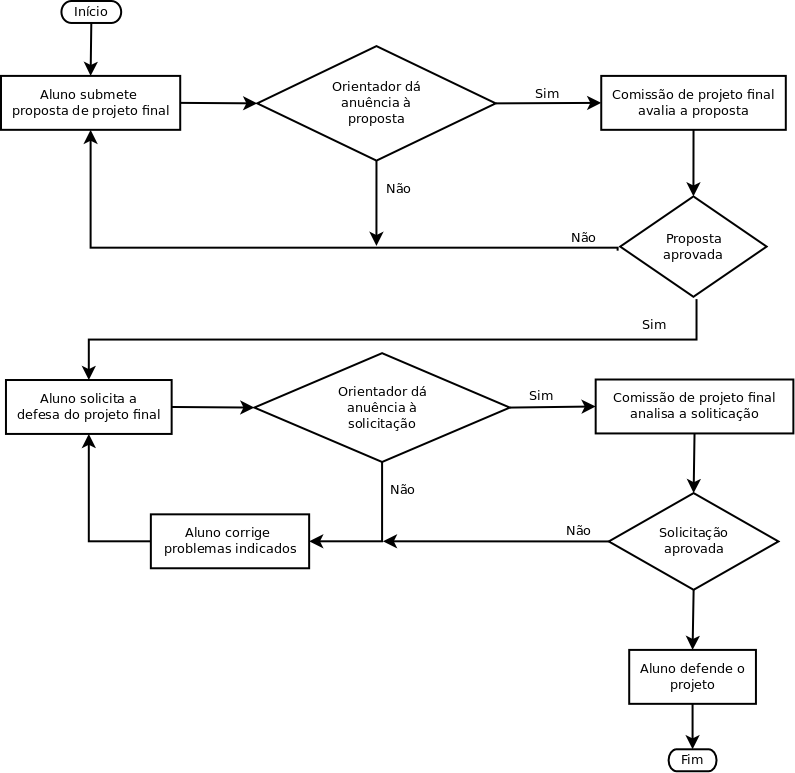
\includegraphics[width=1\textwidth]{fig/fluxograma_tcc.png}
\caption{Fluxograma do desenvolvimento do projeto final}
\label{fig:flux_tcc}
\end{figure}


